\section{Results}

 %\begin{wrapfigure}{r}{0.4\columnwidth}
 %   \vspace{-3em}
 %   	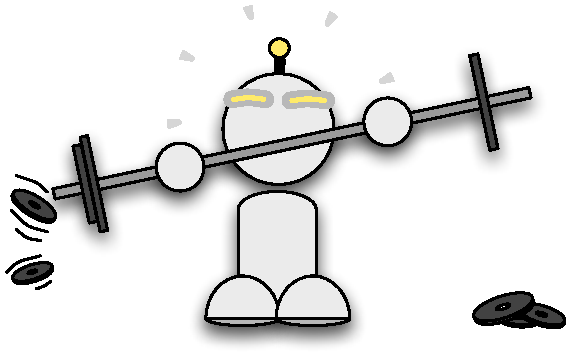
\includegraphics[width=0.3\columnwidth, trim=0mm 10mm 0mm 0mm]{diagrams/robot_weights.pdf}
 %\end{wrapfigure}
\textbf{Figure \ref{fig:speedup}} summarises our \textbf{main result} while Figure
4 and Figure 5 show the amount of improvement we
can regularly obtain. We evaluate performance by running the well known A* algorithm on a range of realistic and synthetic benchmarks:
\begin{itemize}
\item{
\textbf{Adaptive Depth} is a set of 12 maps of size 100$\times$100 which are
composed of rectangular rooms and large open areas containing randomly placed obstacles.
}
\item{
\textbf{Baldur's Gate} is a set of 120 maps taken from BioWare's popular
roleplaying game \emph{Baldurs Gate II: Shadows of Amn}. 
These maps range in size from 50$\times$50 to 320$\times$320.
}
\item{
\textbf{Rooms} is a set of 300 maps of size 256$\times$256 which are divided into 32$\times$32
rectangular areas that are connected by randomly placed entrances.
}
\end{itemize}


% \begin{wrapfigure}{l}{0.3\columnwidth}
%		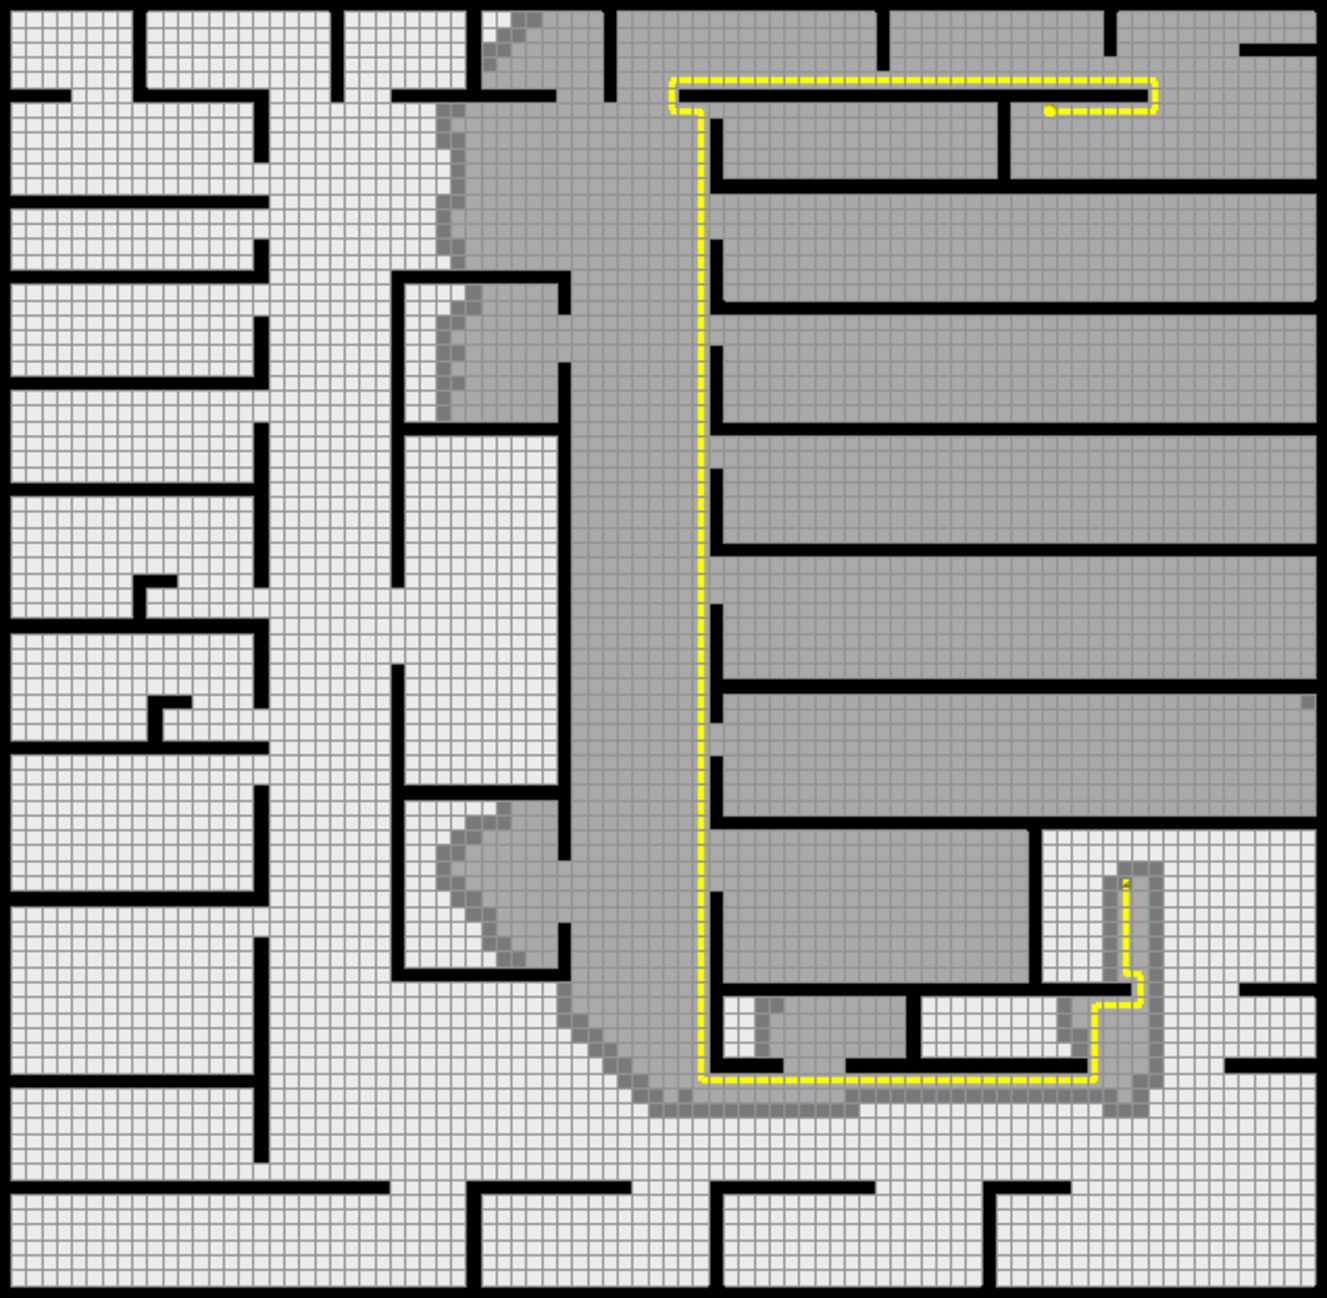
\includegraphics[width=0.3\columnwidth]{diagrams/astarsearch.pdf}
%		\caption{Tiles explored before symmetry elimination.}
% \end{wrapfigure}
% \begin{wrapfigure}{l}{0.3\columnwidth}
%		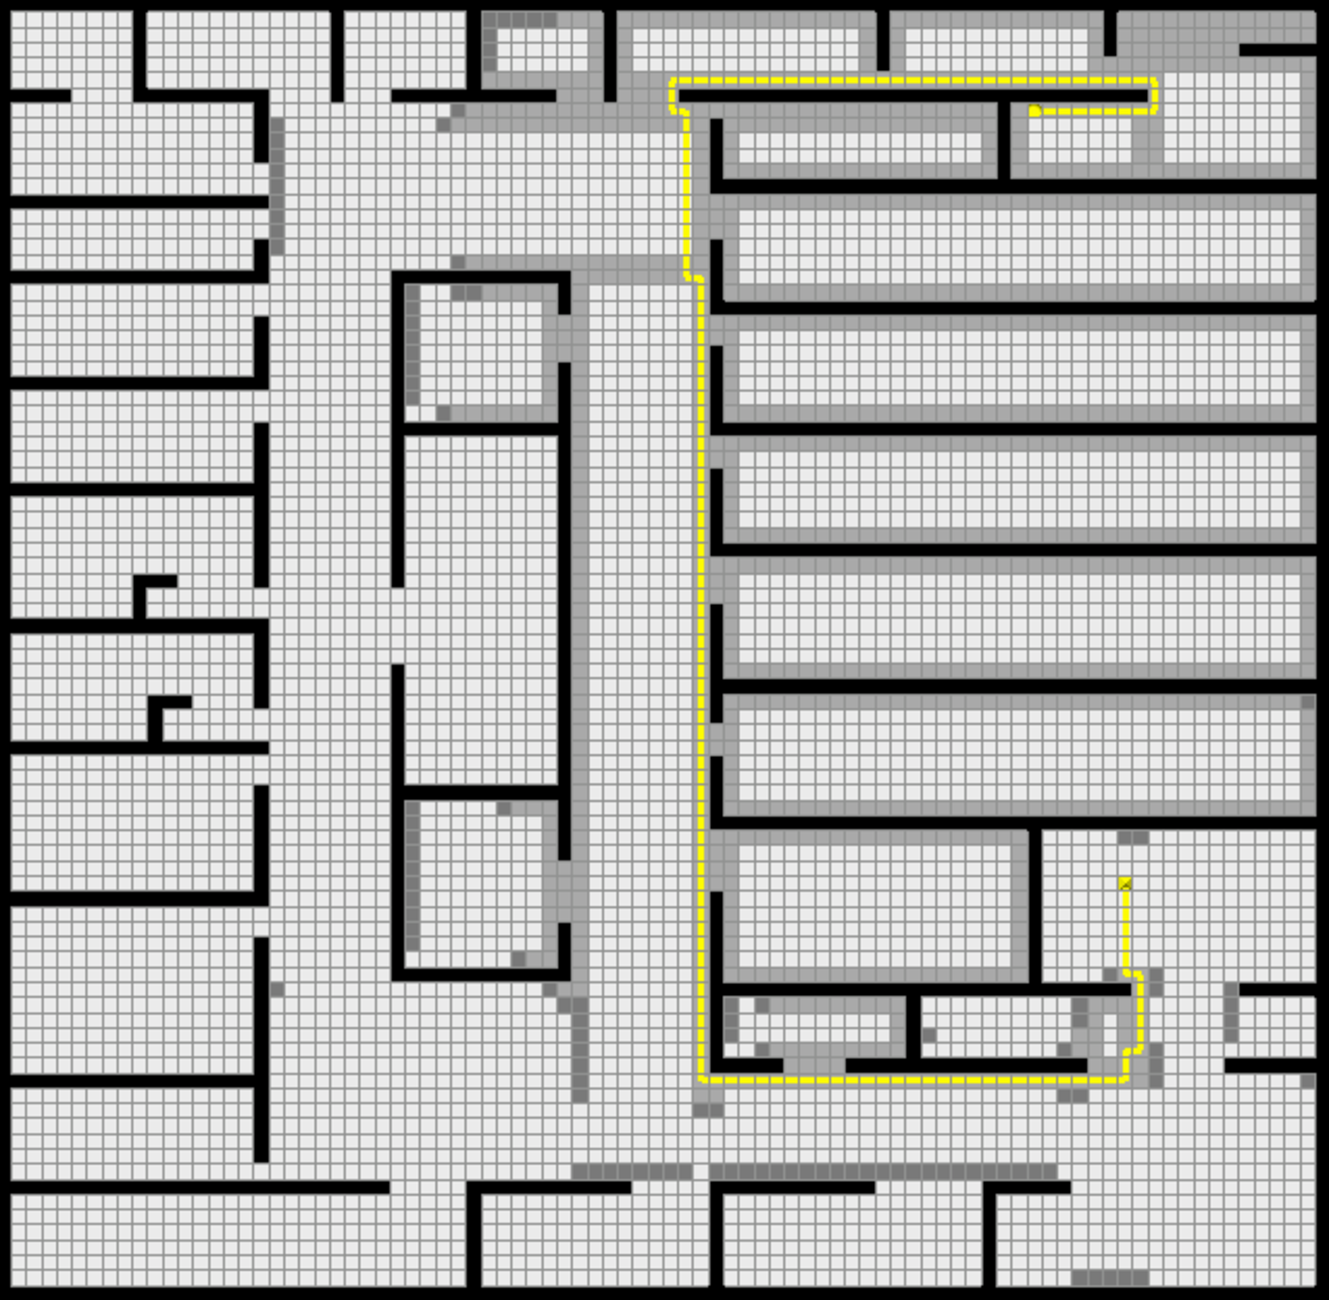
\includegraphics[width=0.3\columnwidth]{diagrams/psearch.pdf}
%		\caption{Tiles explored after symmetry elimination.}
% \end{wrapfigure}
\vspace{1em}
\begin{figure}[h]
\label{fig:speedup}
\begin{center}
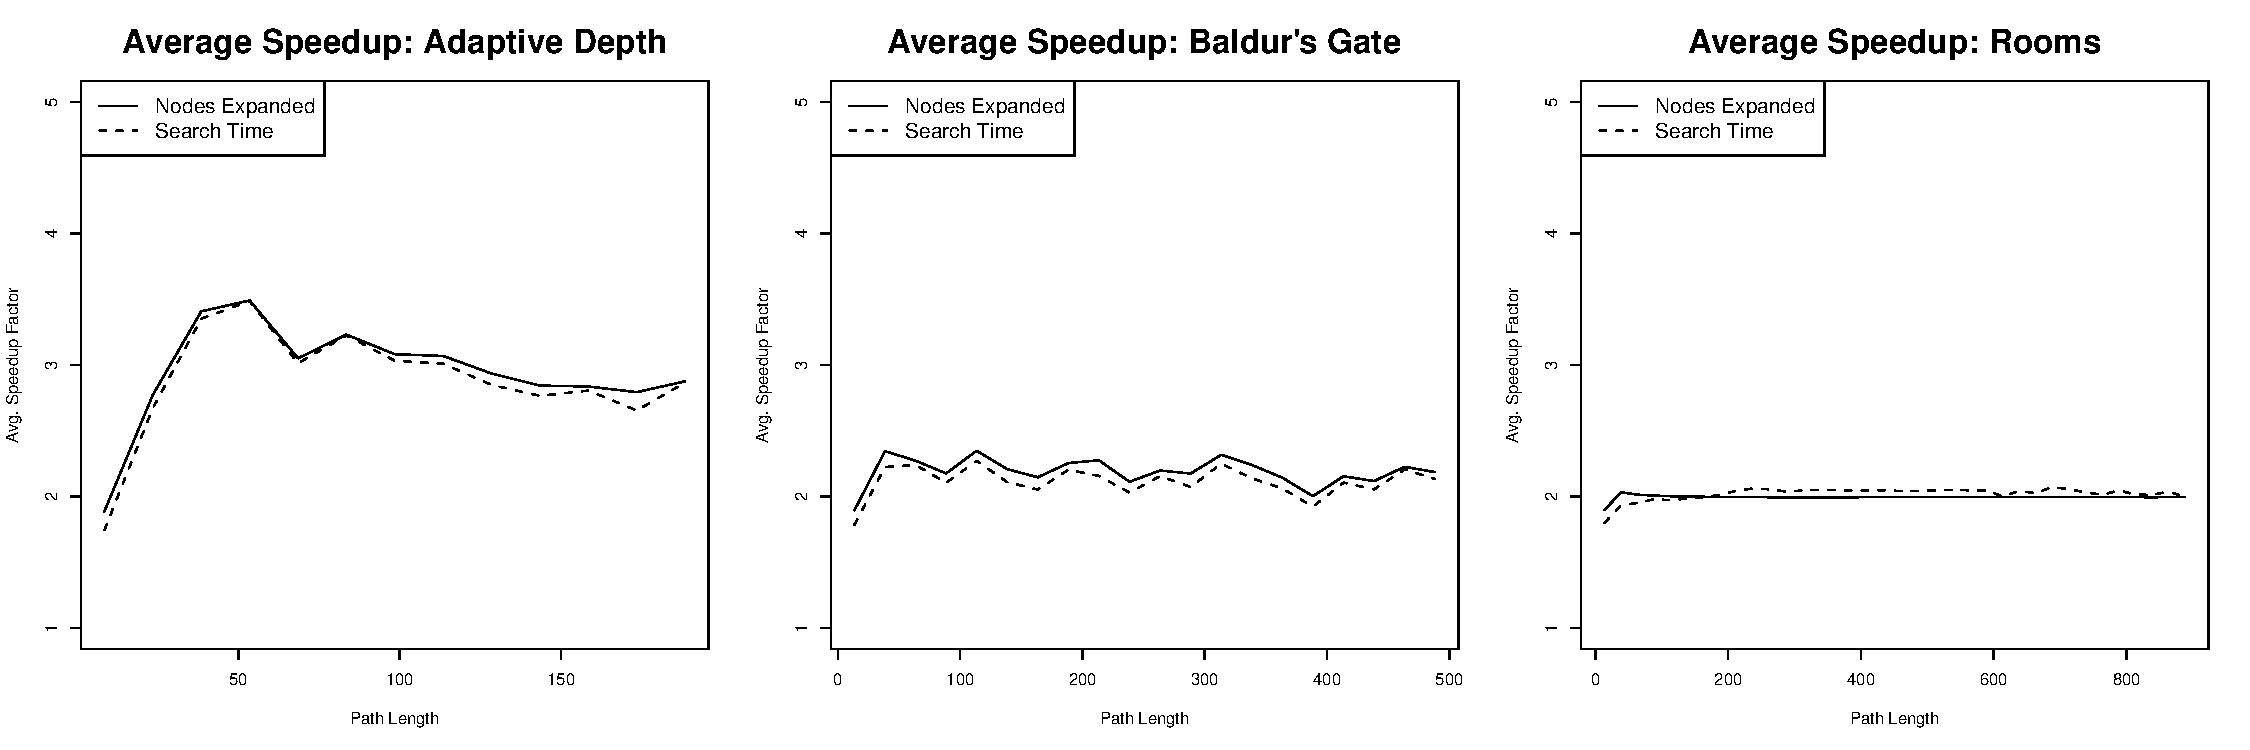
\includegraphics[width=\columnwidth]{diagrams/speedup}
\caption{Using symmetry elimination A* runs between 2-4 times faster on a range of synthetic
and realistic benchmarks.
The best results are achieved on maps with large open areas where we eliminate
many symmetric paths.}
\end{center}
\end{figure}

\begin{figure}
  \begin{minipage}{0.328\columnwidth}
	\label{fig:astar}
	\centering
		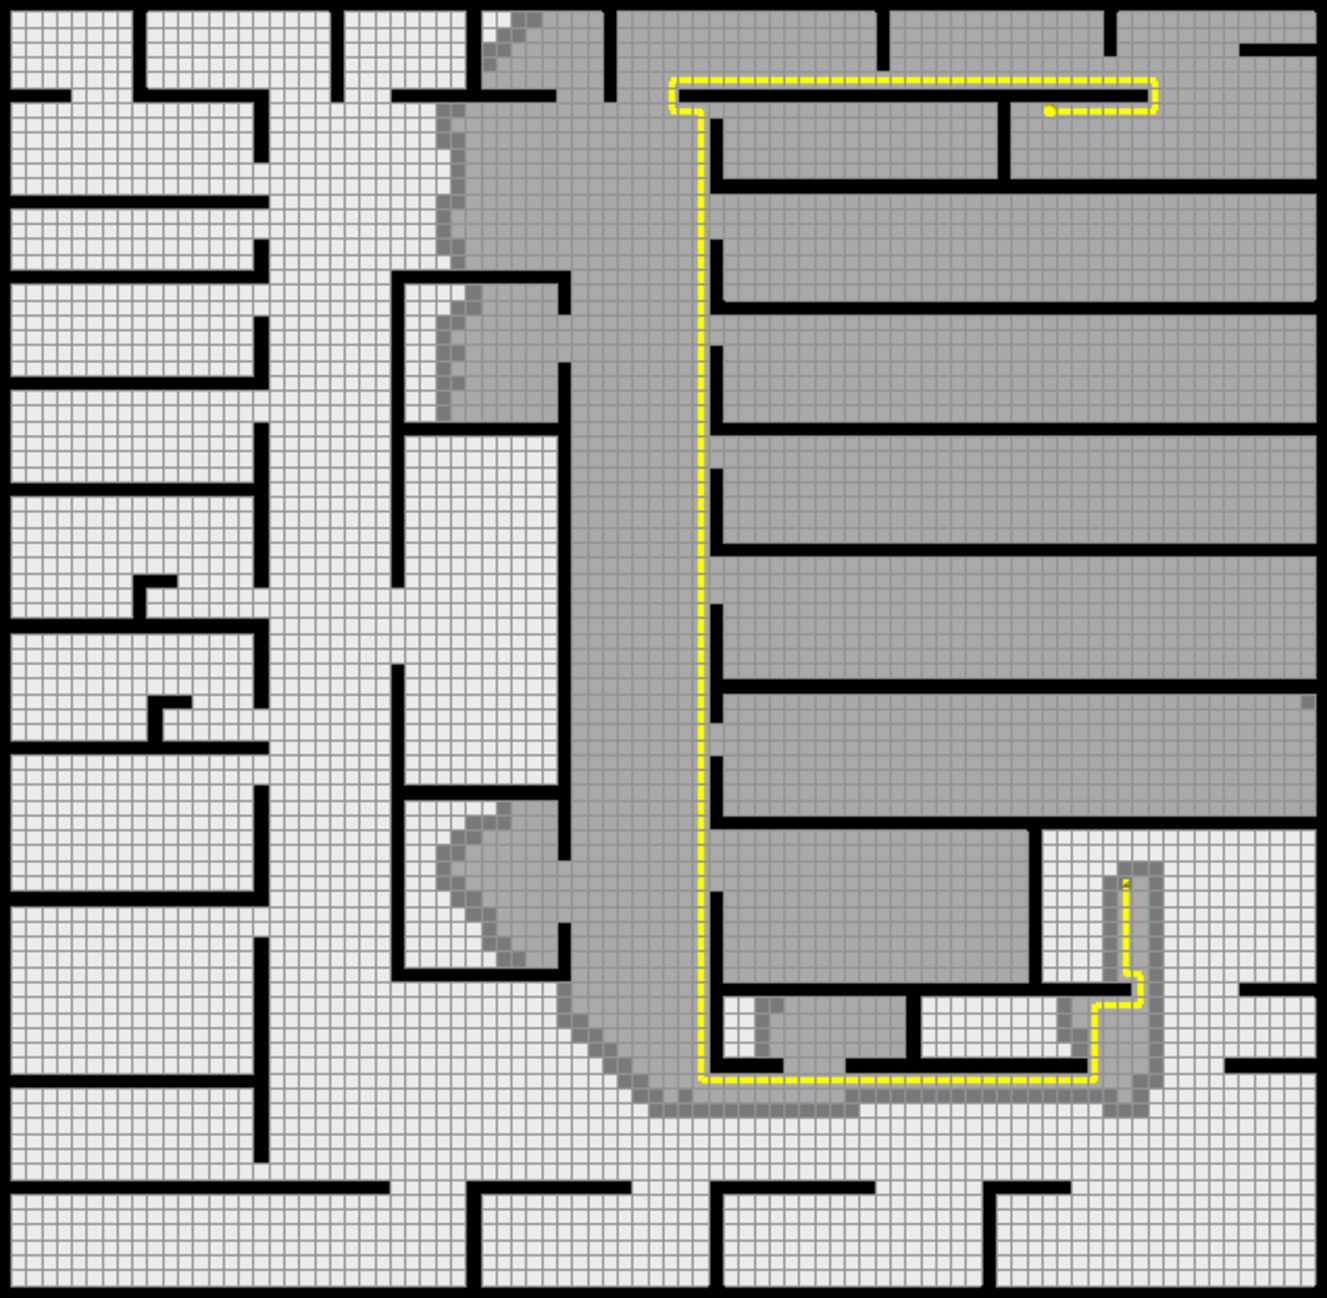
\includegraphics[width=\columnwidth]{diagrams/astarsearch.pdf}
		\caption{Tiles explored before symmetry elimination.}
	\end{minipage}
	\hspace{1em}
	\begin{minipage}{0.33\columnwidth}
	\label{fig:psearch}
		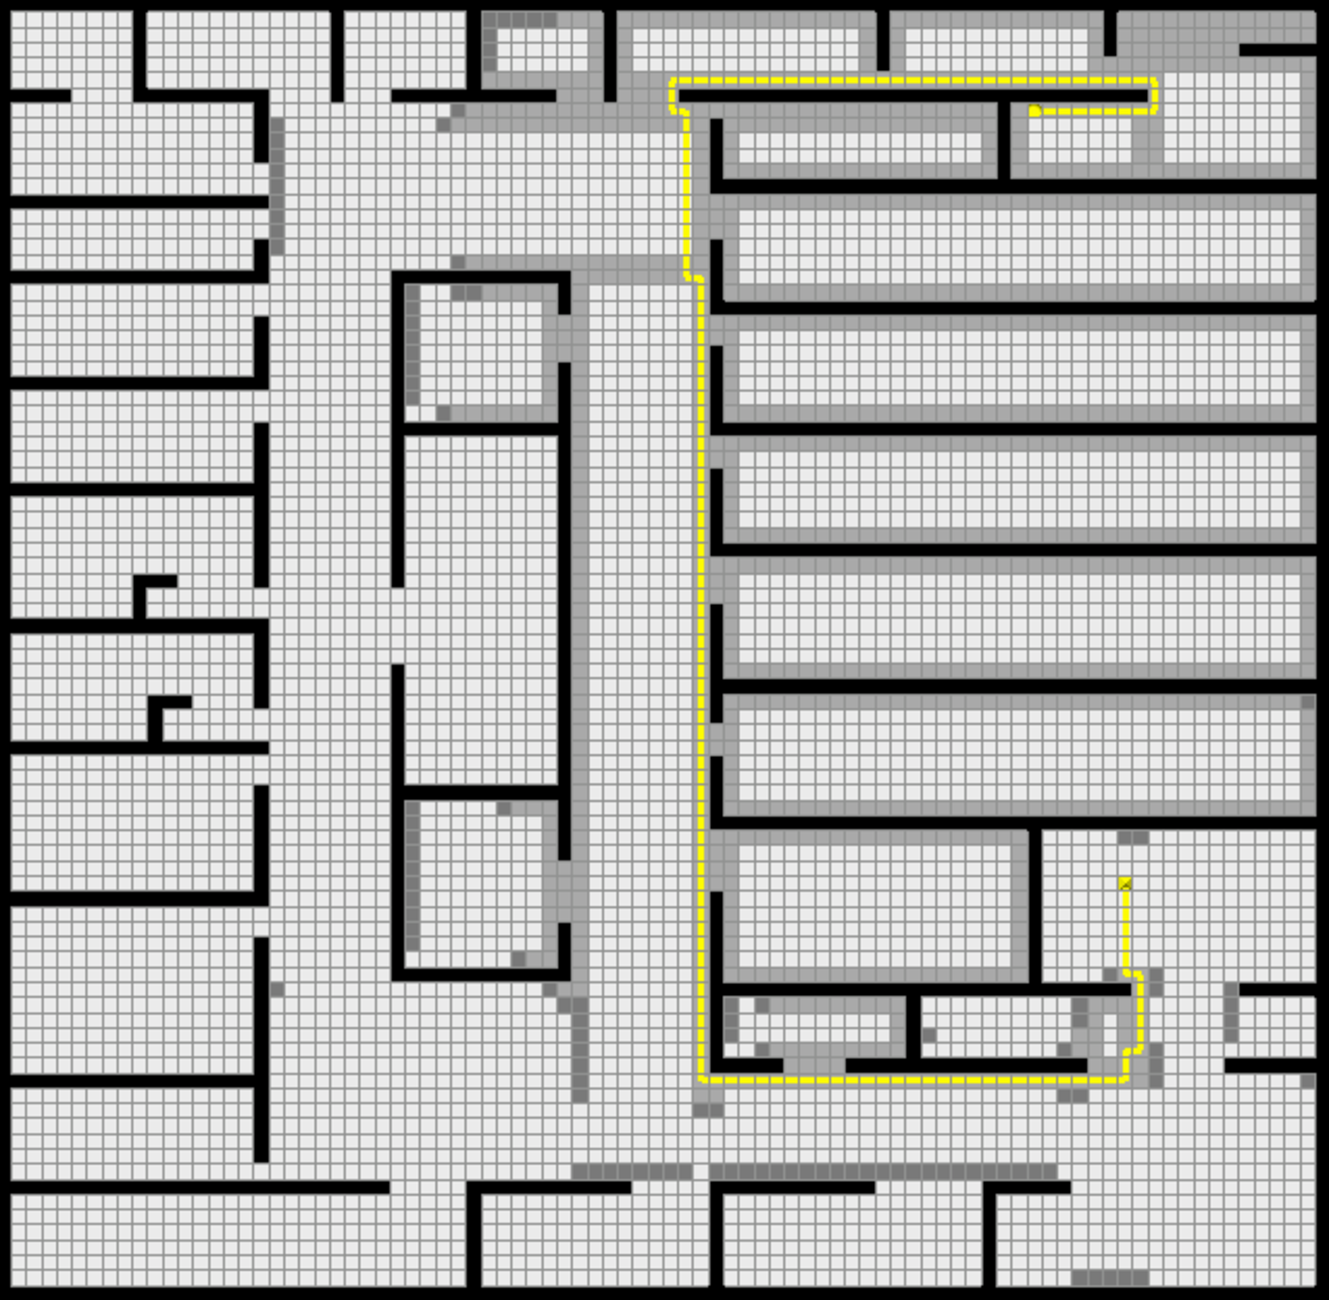
\includegraphics[width=\columnwidth]{diagrams/psearch.pdf}
	\caption{Tiles explored after symmetry elimination.}
	\end{minipage}
\vspace{2em}
 \end{figure}

